\documentclass[12pt]{article}
\usepackage[utf8]{inputenc}
\usepackage[T1]{fontenc}
\usepackage{fontspec}
\setmainfont{Times New Roman}
\newfontfamily\hackfont{Hack}
\usepackage{titlesec}
\usepackage{fancyhdr}
\usepackage{listings}
\usepackage{xcolor}
\usepackage{graphicx}
\usepackage{longtable}
\usepackage{caption}
\usepackage{hyperref}
\usepackage{setspace}
\usepackage{geometry}
\geometry{a4paper, margin=1in}
\hypersetup{colorlinks=true, linkcolor=blue, urlcolor=blue}
\renewcommand{\contentsname}{Table of Contents}

\pagestyle{fancy}
\fancyhf{} 							% Header Middle
\rhead{Shell Programming \& Linux Commands}
\lhead{Operating System–Final Lab Test}
\rfoot{\thepage}

\begin{document}

\begin{titlepage}					% Cover Start
\begin{center}
    
\includegraphics[width=0.35\textwidth]{logo.png} \\
    \vspace{0.5cm}
    \textbf{\Huge \textcolor{teal}{NOTRE DAME} \textcolor{teal}{UNIVERSITY}} \\
    \vspace{0.5cm}
    \textbf{\Huge \textcolor{orange}{BANGLADESH}} \\
    
    \vspace{0.9cm}
    \textbf{\Huge \underline{Operating System Final Lab Test}} \\
    
    \vspace{1.5em}
    \begin{flushleft}
    	\textbf{\Large Course Code: CSE-3206} \\
		\vspace{0.3cm}        
        \textbf{\Large Course Title: Operating System Lab} \\
        \vspace{0.3cm}
        \textbf{\Large Lab Task Topic: Shell Programming \& Linux Commands} \\        
    \end{flushleft}
    
    \vspace{1em}
    \begin{flushleft}
        \textbf{\Huge \textcolor{blue}{Submitted by:}} \\
        \vspace{0.3cm}
        \textbf{\Large Name: Istiak Alam} \\
        \vspace{0.3cm}
        \textbf{\Large ID: 0692230005101005} \\
		\vspace{0.3cm}        
        \textbf{\Large Batch: CSE-20} \\
        \vspace{0.5cm}
        \textbf{\Large Submission Date: }{\Large \textbf{\today}\par}
    \end{flushleft}
    \vfill
    \begin{flushleft}
        \textbf{\Huge \textcolor{blue}{Submitted to:}} \\
        \vspace{0.3cm}
        \textbf{\Large Khorshed Alam} \\
        \vspace{0.3cm}
        \textbf{\Large Lecturer,} \\
        \vspace{0.3cm}
        \textbf{\Large Notre Dame University Bangladesh}
    \end{flushleft}
\end{center}
\end{titlepage}						% Cover End

%\tableofcontents
\thispagestyle{empty}
\clearpage
\pagenumbering{arabic}

\section*{Question 01. Linux Commands}

\textbf{a) List all files and directories, including hidden ones, in the current directory.}
\begin{lstlisting}[language=bash]
$ ls -a
\end{lstlisting}
\vspace{1em}
\noindent\textbf{Output in \texttt{Linux Terminal} :}
\begin{center}
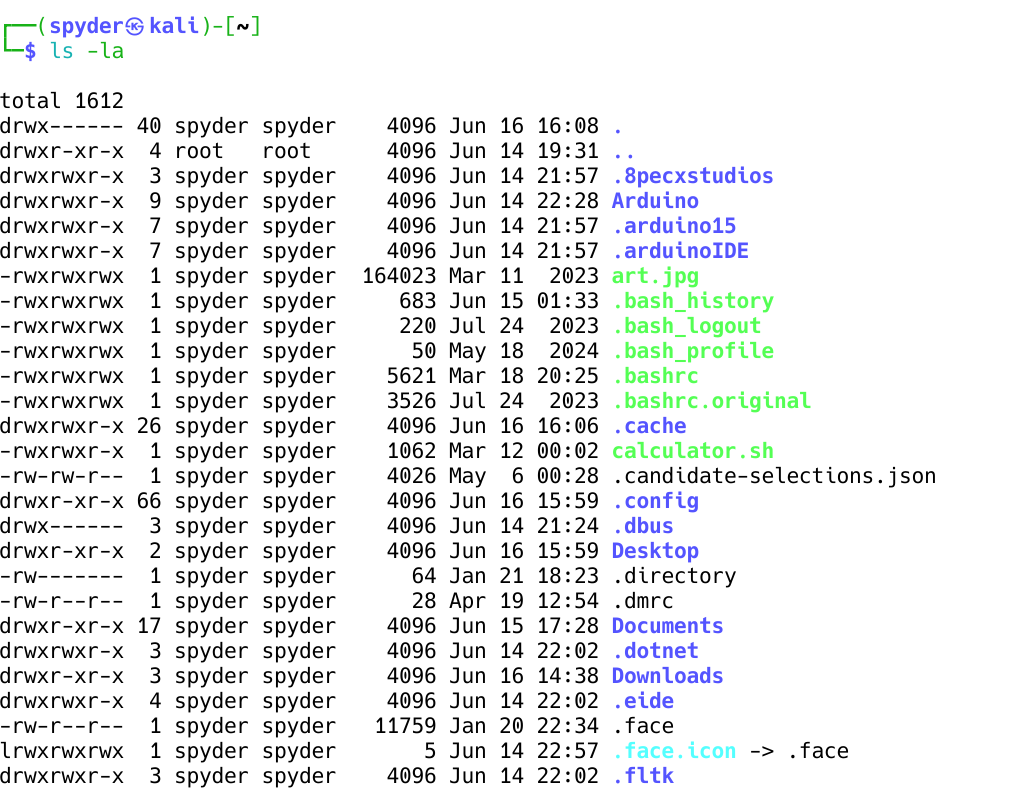
\includegraphics[width=0.8\textwidth]{1.png}
\end{center}
\textbf{b) Count the number of lines, words, and characters in a file named \texttt{sample.txt}.}
\begin{lstlisting}[language=bash]
$ wc sample.txt
\end{lstlisting}
\vspace{1em}
\noindent\textbf{Output in \texttt{Linux Terminal} :}
\begin{center}
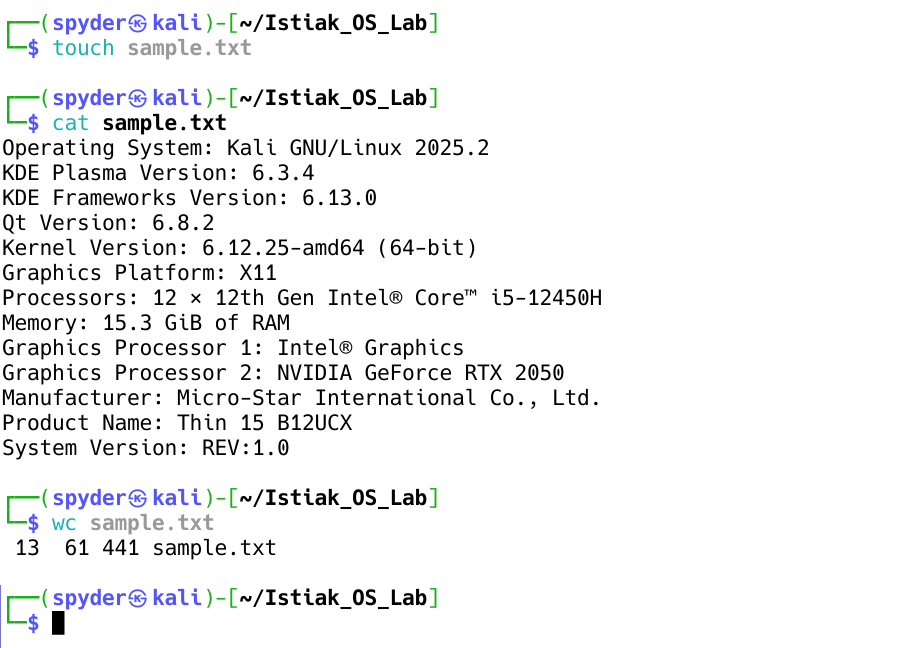
\includegraphics[width=0.7\textwidth]{2.png}
\end{center}
\textbf{c) Display all lines that contain the word \texttt{ERROR} from \texttt{log.txt}.}
\begin{lstlisting}[language=bash]
grep 'ERROR' log.txt
\end{lstlisting}

\vspace{1em}
\noindent\textbf{Sample \texttt{log.txt} Content:}
\begin{lstlisting}[language=bash]
[INFO] System boot completed successfully.
[INFO] User logged in: Istiaq-Alam
[WARNING] Disk space running low on /dev/sda1
[ERROR] Failed to load configuration file: config.yaml
[INFO] Background services started.
[ERROR] Unable to connect to database server.
[DEBUG] Cache initialized.
[INFO] Update check completed.
[ERROR] Invalid user input on form submission.
[INFO] Scheduled backup completed.
\end{lstlisting}

\vspace{1em}
\noindent\textbf{Output in \texttt{Linux Terminal} :}
\begin{center}
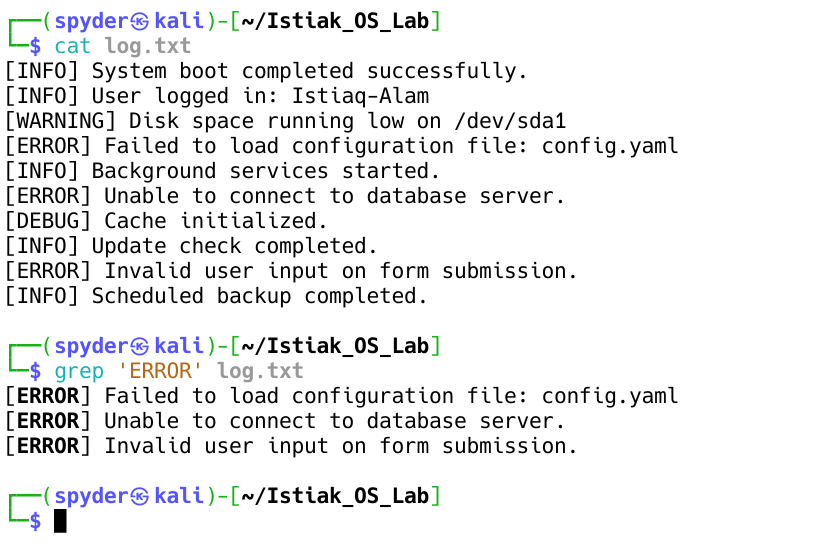
\includegraphics[width=1\textwidth]{3.png}
\end{center}

\newpage

\section*{Question 02. Basic Shell Script}

\textbf{Objective:} A shell script that takes a file name as input and performs the following:

\begin{itemize}
  \item Checks if the file exists.
  \item Displays the number of lines, words, and characters.
  \item Shows the first 5 lines and last 5 lines.
\end{itemize}
\textbf{Shell Script:}
\begin{verbatim}
#!/bin/bash
# Take file name as input
echo "Enter filename:"
read filename
# Check if file exists
if [ -f "$filename" ]; then
    echo "File exists: $filename"    
    # Display number of lines, words, and characters
    echo "Lines, Words, Characters:"
    wc "$filename"
    echo -e "\n--- First 5 Lines ---"
    head -n 5 "$filename"
    echo -e "\n--- Last 5 Lines ---"
    tail -n 5 "$filename"
else
    echo "File not found!"
fi
\end{verbatim}
\vspace{1em}
\noindent\textbf{Output in \texttt{Linux Terminal} :}
\begin{center}
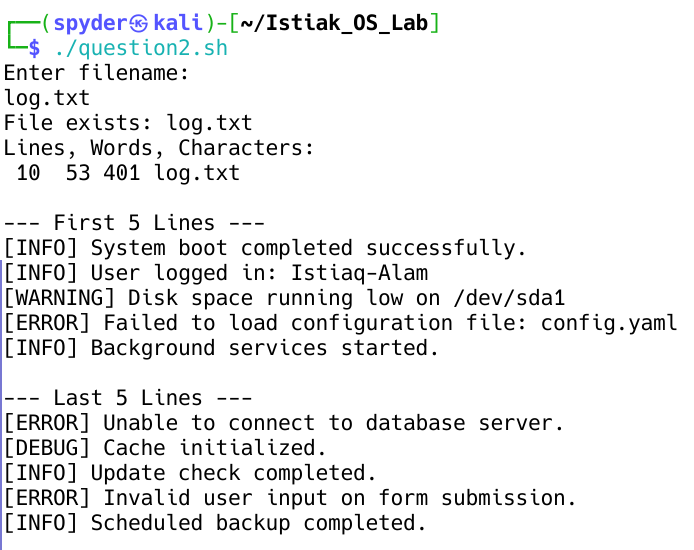
\includegraphics[width=0.7\textwidth]{4.png}
\end{center}

\newpage

\section*{Question 03. Shell Script Using Conditional and Loop}

\textbf{Objective:} A shell script that:
\begin{itemize}
  \item Prompts the user to input a number.
  \item Checks whether the number is a prime number.
  \item Displays a message indicating the result.
  \item Includes input validation and comments.
\end{itemize}
\textbf{Shell Script: [primenum.sh]}
\begin{verbatim}
#!/bin/bash
# Prompt for input
read -p "Enter a number: " num
# Check if input is a valid integer
if ! [[ "$num" =~ ^[0-9]+$ ]]; then
    echo "Invalid input. Please enter a positive integer."
    exit 1
fi
# 0 and 1 are not prime numbers
if [ "$num" -lt 2 ]; then
    echo "$num is not a prime number."
    exit 0
fi
# Prime check using loop
is_prime=1
for (( i=2; i*i<=num; i++ ))
do
    if [ $((num % i)) -eq 0 ]; then
        is_prime=0
        break
    fi
done
# Result
if [ $is_prime -eq 1 ]; then
    echo "$num is a prime number."
else
    echo "$num is not a prime number."
fi
\end{verbatim}
\vspace{2em}
\hrule
\vspace{1em}
\noindent\textbf{Note:} All shell scripts are tested in a Linux environment (e.g., Kali Linux). Make sure to give execution permissions using \texttt{sudo chmod +x primenum.sh} before running.
\vspace{1em}

\newpage
\noindent\textbf{Output in \texttt{Linux Terminal} :}
\begin{center}
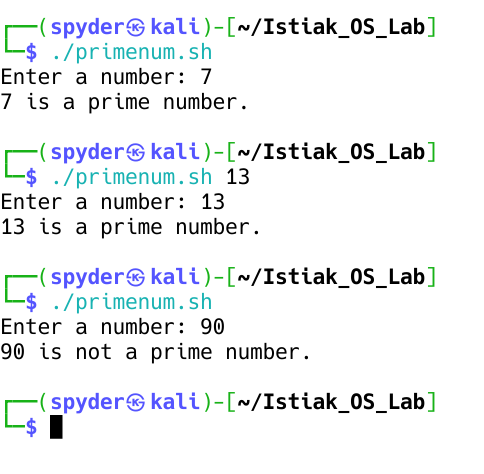
\includegraphics[width=0.6\textwidth]{5.png}
\end{center}

\vspace{9em}
\begin{center}
\Huge THE END
\end{center} 
\end{document}